\chapter{Ergebnisse und Diskussion}

Die Ergebnisse der Analyse der in dieser Arbeit entwickelten FDK-Implementierung werden in diesem Kapitel präsentiert.
Die Implementierung wird außerdem mit den in der Literatur genannten Ergebnissen verglichen.

\section{Leistungsmessung}

Die Analyse der in den vorigen Kapiteln vorgestellten Implementierung des \gls{fdk} erfolgte auf verschiedenen
\gls{gpu}s unterschiedlicher Hardwaregenerationen. Die in den folgenden Abschnitten gezeigten Ergebnisse des Profilings
erfolgten auf einer GeForce GTX 1080, die mit 1733 MHz getaktet ist und über 8 GiB Speicher verfügt. Der Einsatz
mehrerer heterogener \gls{gpu}s erfolgte mit der genannten GeForce GTX 1080 sowie einer Tesla K20c, die eine
Taktfrequenz von 706 MHz sowie 5 GiB Speicher besitzt. Die Untersuchung für homogene \gls{gpu}-Systeme wurde auf
mehreren \gls{gpu}s vom Typ Tesla K80 durchgeführt, die jeweils eine Taktfrequenz von 560 MHz und 12 GiB Speicher
aufweisen. Sofern nicht anders angegeben, wurde stets ein Volumen mit 1070 $\times$ 1070 $\times$ 1033 Voxeln
rekonstruiert.

\subsection{Teilstufen}

Die Analyse des Gesamtprogramms im Profiler, deren Ergebnisse in Tabelle~\ref{tab:op_runtime} zusammengefasst sind,
zeigt, dass die Rückprojektion wie erwartet den größten zeitlichen Anteil der Berechnungen einnimmt. Der Anteil der
restlichen Operationen ist dem gegenüber vernachlässigbar gering. Im Folgenden wird daher nur noch die Rückprojektion
einer genaueren Analyse unterzogen.

\begin{table}
    \centering
    \begin{tabular}{lcc}
        \hline
        Operation & Dauer [s] & Anteil [\%]\\
        \hline
        Gesamtberechnung & 80,356 & 100\\
        Rückprojektion & 79,622 & 99,087\\
        Filterung & 0,631 & 0,786\\
        Wichtung & 0,075 & 0,093 \\
        \texttt{memset} & 0,028 & 0,034\\
        \hline
    \end{tabular}
    \caption{Laufzeiten der einzelnen Operationen auf dem Device\label{tab:op_runtime}}
\end{table}

\subsection{Eigenschaften des Rückprojektionskernels}

In Abschnitt~\ref{ssec:implementierungsidee} wurde als Implementierungsziel unter anderem eine möglichst hohe
\gls{gpu}-Auslastung gefordert. Um diese Auslastung zu erreichen, ist ein möglichst geringer Verbrauch der zwischen den
Threads geteilten Ressourcen erforderlich. Da der geteilte Speicher in der Implementierung nicht verwendet wurde, zielte
die Umsetzung dieser Forderung auf einen möglichst geringen Registerverbrauch ab.

Wie in Abbildung~\ref{fig:kernel_props} zu sehen ist, benötigt der Rückprojektions-\gls{kernel} 19 Register
(grün markiert). Auf der hier verwendeten GeForce GTX 1080 ist somit eine theoretische Auslastung der gesamten \gls{gpu}
möglich, praktisch wird die \gls{gpu} durch die Rückprojektion zu 88,5\% ausgelastet (rot markiert). Das eingangs
gestellte Ziel der hohen Auslastung wurde damit erreicht.

Ein weiteres der in Abschnitt~\ref{ssec:implementierungsidee} genannten Optimierungsziele ist die Verkürzung der
Wartezeit zwischen dem Ende einer Rückprojektion und dem Beginn der nachfolgenden Rückprojektion. Zu diesem Zweck wird
die Rückprojektion in einem eigenen Thread und \gls{cuda}-Stream ausgeführt, sodass die vorherigen Operationen (Laden,
Wichten, Filtern) parallel zur Rückprojektion ausgeführt werden können. Der Rückprojektionsthread entnimmt die nächste
Projektion vom Stapel der noch ausstehenden Projektionen, wandelt diese in eine \gls{cuda}-Textur um und startet dann
den Rückprojektions-\gls{kernel}. Wie Abbildung~\ref{fig:kernel_wait} zeigt, ist es gelungen, die Zeit zwischen zwei
Rückprojektionen, die durch die langen, grün-blauen Balken dargestellt werden, auf 2 Millisekunden zu beschränken. Bei
einem üblichen Datensatz von 1440 Projektionen ergibt sich also eine Gesamtwartezeit von 2,88 Sekunden.

Abbildung~\ref{fig:kernel_wait} zeigt allerdings auch, dass diese Wartezeit noch nicht ideal ist. Das Ziel, die Wichtung
und die Filterung, die durch die kleineren, bunten Balken repräsentiert werden, parallel zur Rückprojektion
durchzuführen, konnte nicht erreicht werden. Der Grund dafür ist vermutlich die Anzahl der Threads, die vom
Rückprojektions-\gls{kernel} gestartet werden. Bei einem Volumen mit 1070 $\times$ 1070 $\times$ 1033 \gls{voxel}n,
denen jeweils ein Thread zugeordnet wird, werden 1.182.681.700 Threads benötigt. Die GTX 1080 verfügt über 20 \gls{sm}s,
von denen jeder bis zu 2.048 Threads gleichzeitig ausführen kann und ist somit in der Lage, bis zu 40.960 Threads
gleichzeitig zu verwalten. Die \gls{gpu} ist daher gezwungen, der Rückprojektion alle verfügbaren Threads zuzuweisen,
was zur Folge hat, dass keine weiteren \gls{kernel} ausgeführt werden können. Um eine Reduzierung der gestarteten
Threads zu erreichen und dadurch die parallele Ausführung der Rückprojektion und der anderen Schritte zu ermöglichen,
ist die Übernahme des von Scherl et al.\ vorgestellten Ansatzes denkbar, also die Iteration eines zweidimensionalen
Kernels durch das Volumen (vgl.~\cite{scherlkeck}). Wenn auch die parallele Ausführung der Rückprojektion und der
vorherigen Schritte nicht gelungen ist, ist auf der Abbildung jedoch zu sehen, dass die Ausführung der \gls{kernel} mit
geringerem Ressourcenbedarf sich stellenweise überlappt.

Die Wartezeit zwischen zwei Rückprojektionen, die über die gesamte Laufzeit akkumuliert ca. 3 Sekunden einnimmt, hat
also einen akzeptablen Wert erreicht, der dem alltäglichen Gebrauch nicht im Wege steht. Es ist an dieser Stelle aber
noch Optimierungspotential vorhanden.

\begin{figure}
    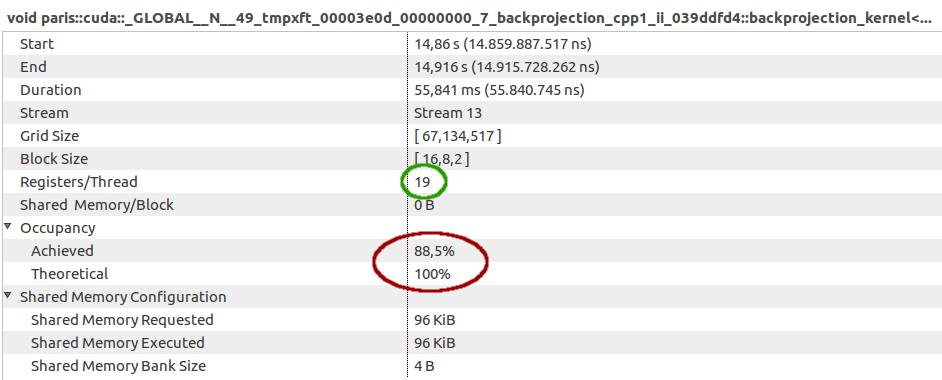
\includegraphics[width=\linewidth]{img/kernel_properties}
    \caption{Eigenschaften des Rückprojektionskernels\label{fig:kernel_props}} 
\end{figure}

\begin{figure}
    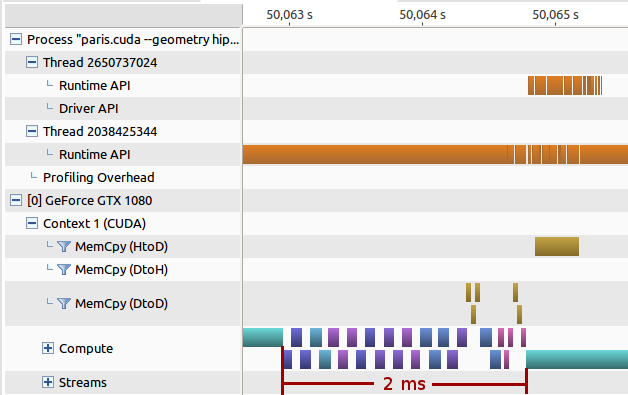
\includegraphics[width=\linewidth]{img/timeline_compute3}
    \caption{Zeit zwischen zwei Rückprojektionen\label{fig:kernel_wait}} 
\end{figure}

\subsection{Laufzeitverhalten}

In Abbildung~\ref{fig:laufzeit_gpu} ist das Laufzeitverhalten der Implementierung angesichts verschiedener Volumengrößen
dargestellt (inklusive Ein- und Ausgabe). Wie man leicht sieht, ist bei kleinen Volumen die Gesamtlaufzeit anscheinend
nicht oder kaum von der Berechnungszeit abhängig. Dies lässt darauf schließen, dass auf der \gls{host}-Seite ein
gewisser Overhead vorhanden ist, der die Rekonstruktion der kleinen Volumen verdeckt. Dies wird noch deutlicher, wenn
man die benötigte Zeit für die Berechnung eines Voxels betrachtet, wie in Abbildung~\ref{fig:voxelzeit} gezeigt. Für
kleine Volumen ist der Zeitbedarf noch relativ hoch. Wird das Volumen größer, fällt zunächst die benötigte Zeit stark ab
und nähert sich im weiteren Verlauf allmählich einem konstanten Wert an. Die Implementierung scheint also besser für
größere als für kleinere Volumen zu skalieren.

\begin{figure}
    \centering
    \begin{tikzpicture}
        \begin{axis}[width=\textwidth,
                     xlabel={Volumengröße [Voxel]},
                     symbolic x coords={133 x 133 x 129,267 x 267 x 258,535 x 535 x 516, 1070 x 1070 x 1033},
                     xtick=data,
                     ylabel={Laufzeit [s]},
                     legend pos=north west]

             \addplot table[x=Volumengroesse,y=GTX1080,col sep=comma] {data/laufzeit.csv};
             \legend{GTX 1080};
        \end{axis}
    \end{tikzpicture}
    \caption{Laufzeit für unterschiedliche Volumengrößen}\label{fig:laufzeit_gpu} 
\end{figure}

\begin{figure}
    \centering
    \begin{tikzpicture}
        \begin{axis}[width=\textwidth,
                     xlabel={Volumengröße [Voxel]},
                     symbolic x coords={133 x 133 x 129,267 x 267 x 258,535 x 535 x 516, 1070 x 1070 x 1033},
                     xtick=data,
                     ylabel={Berechnungszeit [µs]},
                     legend pos=north east]

             \addplot table[x=Volumengroesse,y=GTX1080,col sep=comma] {data/voxel.csv};
             \legend{GTX 1080};
        \end{axis}
    \end{tikzpicture}
    \caption{Berechnungszeit pro Voxel}\label{fig:voxelzeit} 
\end{figure}

\subsection{Mehrere GPUs}

Die parallele Berechnung verschiedener Teile des Volumens durch den Einsatz mehrerer \gls{gpu}s war ebenfalls ein
Implementierungsziel. Die besondere Herausforderung bestand darin, sowohl mehrere \gls{gpu}s des gleichen Typs als auch
unterschiedliche \gls{gpu}s zu unterstützen.

Wie Abbildung~\ref{fig:kernel_multi_compute} zeigt, ist es gelungen, die Ausführung parallel auf mehreren \gls{gpu}s
durchzuführen. Der gewählte Ansatz zur Lastverteilung (siehe Abschnitt~\ref{ssec:implementierungsidee}) führt jedoch bei
unterschiedlich leistungsstarken \gls{gpu}s dazu, dass die stärkere \gls{gpu} vor der schwächeren fertig ist und dann
auf diese warten muss, wie in Abbildung~\ref{fig:kernel_multi_bad} zu sehen ist.

In Abbildung~\ref{fig:laufzeit_gpus_heterogen} ist das Laufzeitverhalten unterschiedlicher \gls{gpu}s dargestellt. Es
ist klar zu sehen, dass der gemeinsame Einsatz der Tesla K20c und der GTX 1080 in diesem Fall sogar zu einer längeren
Laufzeit führt, als der alleinige Einsatz der GTX 1080. Die statische Lastverteilung, wie sie in dieser Arbeit
beschrieben wurde, ist für diesen Anwendungsfall daher nicht optimal. 

Im Gegensatz dazu kann die Implementierung durch den Einsatz mehrerer identischer \gls{gpu}s bei der Berechnung großer
Volumen beschleunigt werden, wie das in Abbildung~\ref{fig:laufzeit_gpus_homogen} dargestellte Laufzeitverhalten zeigt.
Diese Beschleunigung fällt allerdings nicht so stark aus wie erhofft, da die theoretische Halbierung der Laufzeit beim
Einsatz einer weiteren Karte nicht annähernd erreicht wird. Bei kleineren Volumen verlängert sich die Laufzeit im
Vergleich zum Gebrauch einer einzigen Karte sogar. Es ist davon auszugehen, dass der oben erwähnte Overhead auf der
\gls{host}-Seite hier ebenfalls zum Tragen kommt.

\begin{figure}
    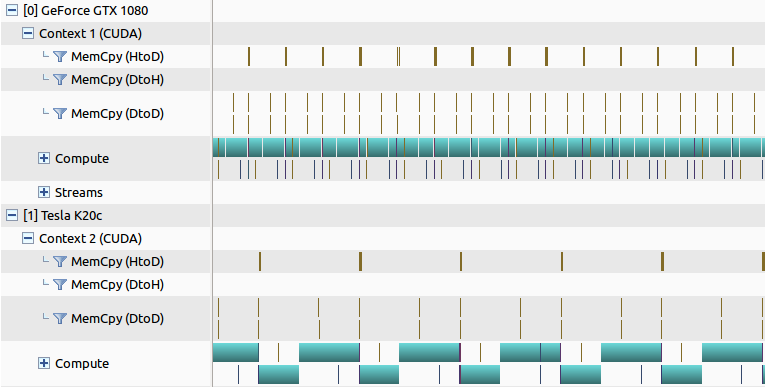
\includegraphics[width=\linewidth]{img/timeline_multi_compute}
    \caption{Parallele Ausführung auf zwei \gls{gpu}s}
    \label{fig:kernel_multi_compute}
\end{figure}

\begin{figure}
    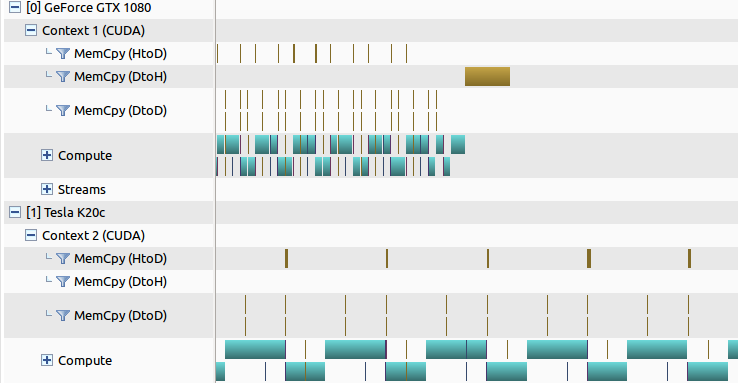
\includegraphics[width=\linewidth]{img/timeline_multi_bad}
    \caption{Der gewählte, statische Lastverteilungsansatz führt zu Wartezeiten}
    \label{fig:kernel_multi_bad}
\end{figure}

\begin{figure}
    \centering
    \begin{tikzpicture}
        \begin{axis}[width=\textwidth,
                     xlabel={Volumengröße [Voxel]},
                     symbolic x coords={133 x 133 x 129,267 x 267 x 258,535 x 535 x 516, 1070 x 1070 x 1033},
                     xtick=data,
                     ylabel={Laufzeit [s]},
                     legend pos=north west]

             \addplot table[x=Volumengroesse,y=GTX1080,col sep=comma] {data/mehreregpusheterogen.csv};
             \addplot table[x=Volumengroesse,y=K20c,col sep=comma] {data/mehreregpusheterogen.csv};
             \addplot table[x=Volumengroesse,y=GTX1080K20c,col sep=comma] {data/mehreregpusheterogen.csv};
             \legend{GTX 1080,Tesla K20c,GTX \& Tesla};
        \end{axis}
    \end{tikzpicture}
    \caption{Laufzeit mit mehreren, verschiedenen \gls{gpu}s}\label{fig:laufzeit_gpus_heterogen} 
\end{figure}

\begin{figure}
    \centering
    \begin{tikzpicture}
        \begin{axis}[width=\textwidth,
                     xlabel={Volumengröße [Voxel]},
                     symbolic x coords={133 x 133 x 129,267 x 267 x 258,535 x 535 x 516, 1070 x 1070 x 1033},
                     xtick=data,
                     ylabel={Laufzeit [s]},
                     legend pos=north west]

             \addplot table[x=Volumengroesse,y=1xK80,col sep=comma] {data/mehreregpushomogen.csv};
             \addplot table[x=Volumengroesse,y=2xK80,col sep=comma] {data/mehreregpushomogen.csv};
             \addplot table[x=Volumengroesse,y=4xK80,col sep=comma] {data/mehreregpushomogen.csv};
             \legend{1x Tesla K80,2x Tesla K80,4x Tesla K80};
        \end{axis}
    \end{tikzpicture}
    \caption{Laufzeit mit mehreren, identischen \gls{gpu}s}
    \label{fig:laufzeit_gpus_homogen}
\end{figure}


\section{Vergleich mit der Literatur}

Der Vergleich mit den oben vorgestellten Ansätzen der Literatur ist ebenfalls von Interesse. Da Zhao et al.\ in ihrer
Arbeit nur Zeiten für die Rückprojektion angeben, werden im Vergleich mit der von ihnen vorgestellten Variante ebenfalls
nur die Zeiten der Rückprojektion berücksichtigt. Scherl et al.\ beziehen dagegen auch die Datenein- und -ausgabe mit
ein. Zur Messung wurde von Zhao et al.\ die 2007 erschienene NVIDIA Quadro FX4600 eingesetzt, die über 768 MiB Speicher
verfügt; Scherl et al.\ verwendeten die 2006 vorgestellte NVIDIA GeForce 8800 GTX, die ebenfalls mit 768 MiB Speicher
ausgerüstet ist. Für den Vergleich fand in dieser Arbeit die 2016 präsentierte NVIDIA GeForce GTX 1080 Verwendung, die
mit 8 GiB Speicher ausgestattet ist.

Da diese \gls{gpu}s aus unterschiedlichen Hardware-Generationen stammen, ist ein direkter Vergleich der erreichten
Rekonstruktionszeiten nicht sinnvoll. Eine Implementierung und ein Vergleich aller genannten Strategien auf derselben
Hardware geht über den Fokus dieser hinaus; es ist deswegen eine Normierung der Ergebnisse notwendig. Dazu werden die
Literaturergebnisse mit einem auf der jeweiligen Taktfrequenz $T$ beruhenden Faktor $G$ multipliziert, um die Ausführung
auf der GTX 1080, die mit 1733 MHz getaktet ist, zu simulieren:

\begin{equation*}
    G_{\text{GPU}} = \frac{T(\text{GPU})}{1733\ \text{MHz}}
\end{equation*}

Die in Tabelle~\ref{table:paris_vs_scherl_zhao} gezeigten Ergebnisse der Literatur sind mit diesem Faktor normiert
worden. Wie die obere Hälfte der Tabelle~\ref{table:paris_vs_scherl_zhao} zeigt, kann die vorgestellte Implementierung
die von Scherl et al.\ präsentierten Werte, inklusive der Datenein- und Ausgabe, nicht erreichen. Der Grund dafür liegt
wahrscheinlich in der noch nicht optimalen Kommunikation zwischen \gls{host} und \gls{device}, der Ein- und Ausgabe der
Daten oder sonstigem Host-Overhead, da die reine Rückprojektion wesentlich schneller funktioniert, wie die untere
Tabellenhälfte zeigt.

Vergleicht man nur die für die Rückprojektion benötigte Zeit, so konnten die von Zhao et al.\ vorgestellten Zeiten für
kleine Volumen erreicht werden. Die Nutzung der Symmetrien scheint daher für kleinere Volumen keinen wesentlichen
Vorteil zu bieten. Bei größeren Volumen ist der von Zhao et al.\ vorgeschlagene Ansatz allerdings um etwa 15\% schneller
als der in dieser Arbeit verfolgte. Die Verwendung dieses Ansatzes birgt also in Fällen, in denen alle für die Nutzung
von Symmetrien notwendigen Projektionen vorliegen, weiteres Potential zur Optimierung.

\begin{table}
    \centering
    \begin{tabular}{llccc}
        \hline
        & GPU & Volumengröße [Voxel] & Projektionszahl & Zeitbedarf [s]\\
        \hline
        Scherl et al. & GeForce 8800 GTX & 512 $\times$ 512 $\times$ 512 & 414 & 4\\
        Stephan & GeForce GTX 1080 & 512 $\times$ 512 $\times$ 512 & 360 & 9\\
        Stephan & GeForce GTX 1080 & 512 $\times$ 512 $\times$ 512 & 480 & 9\\
        \hline
        Zhao et al. & Quadro FX4600 & 512 $\times$ 512 $\times$ 512 & 360 & 2\\
        Stephan & GeForce GTX 1080 & 512 $\times$ 512 $\times$ 512 & 360 & 2\\
        Zhao et al. & Quadro FX4600 & 1024 $\times$ 1024 $\times$ 1024 & 720 & 29\\
        Stephan & GeForce GTX 1080 & 1024 $\times$ 1024 $\times$ 1024 & 720 & 34\\
        \hline
    \end{tabular}
    \caption{Vergleich mit denen von Scherl et al.\ und Zhao et al.\ vorgestellten Ansätzen}
    \label{table:paris_vs_scherl_zhao}
\end{table}
